\documentclass{beamer}

% For more themes, color themes and font themes, see:
% http://deic.uab.es/~iblanes/beamer_gallery/index_by_theme.html
%
\mode<presentation>
{
	\usetheme{Madrid}       % or try default, Darmstadt, Warsaw, ...
	\usecolortheme{default} % or try albatross, beaver, crane, ...
	\usefonttheme{serif}    % or try default, structurebold, ...
	\setbeamertemplate{navigation symbols}{}
	\setbeamertemplate{caption}[numbered]
} 

%\usepackage[english]{babel}
%\usepackage[utf8x]{inputenc}
\usepackage[russian]{babel}
\usepackage[utf8x]{inputenc}
\usepackage{chemfig}
\usepackage[version=3]{mhchem}
\usepackage{amssymb}
\usepackage[ampersand]{easylist}
\usepackage{graphicx}
\graphicspath{{pictures/}}
\DeclareGraphicsExtensions{.pdf,.png,.jpg}

% On Overleaf, these lines give you sharper preview images.
% You might want to `comment them out before you export, though.
\usepackage{pgfpages}
\pgfpagesuselayout{resize to}[%
physical paper width=8in, physical paper height=6in]

% Here's where the presentation starts, with the info for the title slide
\title[Неконтролируемое обучение]{Кластеризация изображений по визуальному подобию с помощью вариационных автоэнкодеров}
\author[А.С. Коваленко]{А. С. Коваленко}
\institute[ЮФУ]{ЮФУ\\ Институт математики, механики и комптьютерных наук им. И. И. Воровича
	\\ научный руководитель: доцент кафедры ПМП, к.ф.-м.н. Я. М. Демяненко}
\date{\today}
\subject{Computer Science}

\newcommand\myitemize{\ListProperties(Hide=100, Hang=true, Progressive=3ex, Style*=$\star$ )}
\newcommand\myenumerate{\ListProperties(Space=2\baselineskip)}
\setbeamertemplate{bibliography item}{}


\begin{document}
	
	\begin{frame}
	\titlepage
\end{frame}

% These three lines create an automatically generated table of contents.
\begin{frame}{Содержание}
\tableofcontents
\end{frame}

\section{Введение}

\subsection{Постановка задачи}
\begin{frame}{Введение}{Постановка задачи}
Разметка данных всегда трудоемкий процесс. Поэтому алгоритмы машинного обучения не требующие данного этапа актуальны. Класс вариационных автоэнкодеров позволяет решить данную проблему.\\

\begin{block}{Поставим задачу:}
Пусть имеется набор изображений:
\begin{equation}\label{eq:X}
X = \{I_m\}_{m = 1}^{N}
\end{equation}
Требуется разбить данный набор на \textit{K} классов и ввести операцию сравнения.\\
Для произвольного изображения найдем \textit{M} схожих объектов из множества \textit{X}, отсортированных по убыванию визуального подобия:
$$I_{input} \notin X,  S = \{I_{m_k}\}_{k=1}^M$$
\end{block}

\end{frame}

\subsection{Обзор подходящих алгоритмов}



\begin{frame}{Введение}{Обзор подходящих алгоритмов}

Для решения поставленной задачи могут подойти следующие подходы неконтролируемого обучения и обучения с подкреплением:
\begin{itemize}
\item Сиамские нейронные сети
\item Ключевые точки (не является алгоритмом машинного обучения)
\item Автоэнкодеры
\end{itemize}

\end{frame}

\begin{frame}{Введение}{Обзор подходящих алгоритмов}

Для решения поставленной задачи могут подойти следующие подходы неконтролируемого обучения и обучения с подкреплением:
\begin{itemize}
\item Сиамские нейронные сети
\item Ключевые точки (не является алгоритмом машинного обучения)
\begin{block}
\item Автоэнкодеры
\end{block}
\end{itemize}

\end{frame}

\section{Автоэнкодеры}

\subsection{Принцип работы}


\begin{frame}{Автоэнкодеры}{Принцип работы}

\begin{block}{Определение:}
\textbf{Автоэнкодеры} --- это нейронные сети прямого распространения, которые восстанавливают входной сигнал на выходе.
\end{block}

\begin{figure}[h]
\center{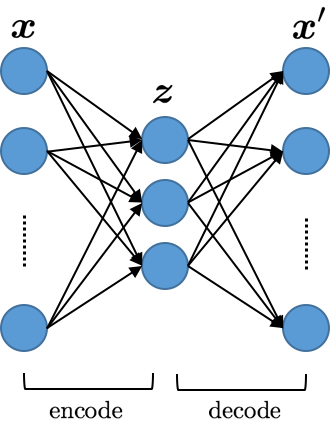
\includegraphics[scale=0.7]{ae}}
\label{fig:ae}
\end{figure}

\end{frame}

\begin{frame}{Автоэнкодеры}{Принцип работы}

\begin{minipage}{0.4\textwidth}
\begin{flushleft}
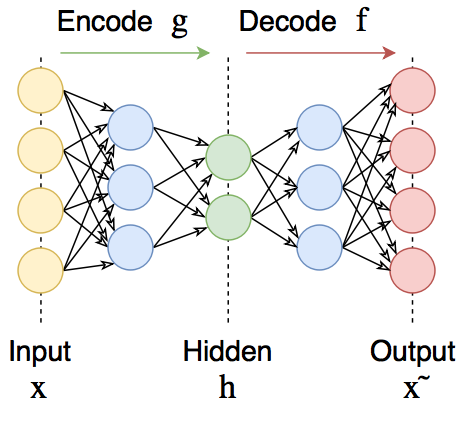
\includegraphics[scale=0.35]{ae_1}
\end{flushleft}
\end{minipage}
\hfill
\begin{minipage}{0.4\textwidth}
\begin{center}
$$g - \text{энкордер}, ~f - \text{декодер},$$
$$x - \text{сигнал}, ~h - \text{код сигнала}$$
$$h = g(x), ~x = f(h)$$
\begin{equation}\label{eq:aim_func}
x = f(g(x))
\end{equation}
\end{center}
\end{minipage}

\end{frame}

\subsection{Разряженные автоэнкодеры}

\begin{frame}{Автоэнкодеры}{Разряженные автоэнкодеры}
Автоэнкодер при обучении стремится аппроксимировать \text{функцию ~(\ref{eq:aim_func}):} $$x = f(g(x)),$$ минимизируя заданный функционал ошибки:
\begin{equation}\label{eq:L}
\min_{\omega} L(x, f(g(x))),
\end{equation}
где $\omega$ - параметры автоэнкодера

\begin{block}{Определение:}
\textbf{Разряженным} называется автоэнкодер, для которого критерий обучения включает также минимизацию разреженности $\Omega(h)$ на кодовом слове $h$:
$$\min_{\omega} L(x, f(g(x))) + \Omega(h),$$
где $\Omega(h)$ - обычный регуляризатор (пусть $L_1$), $\Omega(h) = \lambda*\|h\|$
\end{block}

\end{frame}

\subsection{Вариационные автоэнкодеры}

\begin{frame}{Автоэнкодеры}{Вариационные автоэнкодеры}
Рассмотрим работу декодера как некоторый процесс генерации данных $X$, зависящий от скрытых переменных $Z$ - случайных величин.\\
Пусть:
\begin{itemize}
\item $P(X)$ - вероятностное распределение изображений
\item $P(Z)$ - вероятностное распределение скрытых переменных
\item $P(Z|X)$ - вероятностное распределение скрытых параметров при заданном изображении $X$, рассматривается как энкодер
\item $P(X|Z)$ - вероятностное распределение изображений при заданных скрытых переменных $Z$, рассматривается как декодер
\end{itemize}
\end{frame}

\begin{frame}{Автоэнкодеры}{Вариационные автоэнкодеры}
Справедливо:
\begin{equation}\label{eq:int}
P(X) = \int_{Z} P(X|Z)P(Z) dZ
\end{equation}
Пространство может быть высокоразмерным, поэтому напрямую хорошо приблизить интеграл не получится. Воспользуемся тем, что для заданного X соответствует небольшое подмножество Z, а для остальных вероятность $P(X|Z) \to 0$. Также при приближении будем семплировать из ``оптимальных'' $Z$. \par\medskip
Чтобы понимать какие $Z$ ``оптимальные'' вводится распределение $Q(Z|X)$, которое будет показывать для $X$ распределение $Z \thicksim Q$, которое приводит к этому $X$.
\end{frame}

\begin{frame}{Автоэнкодеры}{Вариационные автоэнкодеры}

Пусть $Q(Z|X)$ будет нормальным распределением:
\begin{equation}\label{eq:Q}
Q(Z|X) = N(\mu(X), \Sigma(X)),
\end{equation}
где $\mu$ и $\Sigma$ - среднее и матрица ковариации для нормального распределения. \par\medskip
Таким образом семплирование скрытых параметров идет из нормального распределения с параметрами $\mu$, $\Sigma$. $P(Z|X)$ также является нормальным распределением. \par\medskip
Функционал ошибки для обучения ~(\ref{eq:L}) выводится из рассмотрения расстояния Кульбака-Лейблера между $Q(Z|X)$ и $P(Z|X)$.

\end{frame}

\begin{frame}{Автоэнкодеры}{Вариационные автоэнкодеры}

\begin{figure}[h]
\center{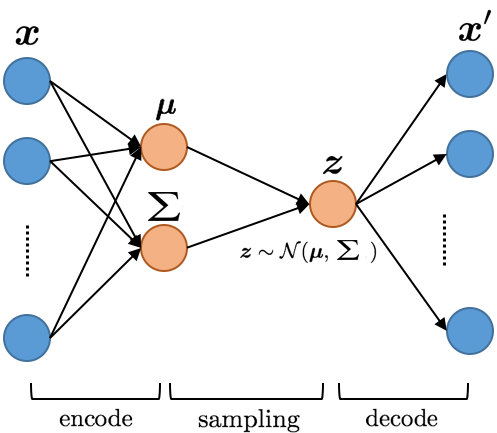
\includegraphics[scale=1]{vae}}
\label{fig:vae}
\end{figure}

\end{frame}

\section{Применение вариационных автоэнкодеров к задаче}

\subsection{Архитектура построенного автоэнкодера}

\begin{frame}{Применение вариационных автоэнкодеров к задаче}{Архитектура построенного автоэнкодера}

\begin{minipage}{0.1\textwidth}
\begin{flushleft}
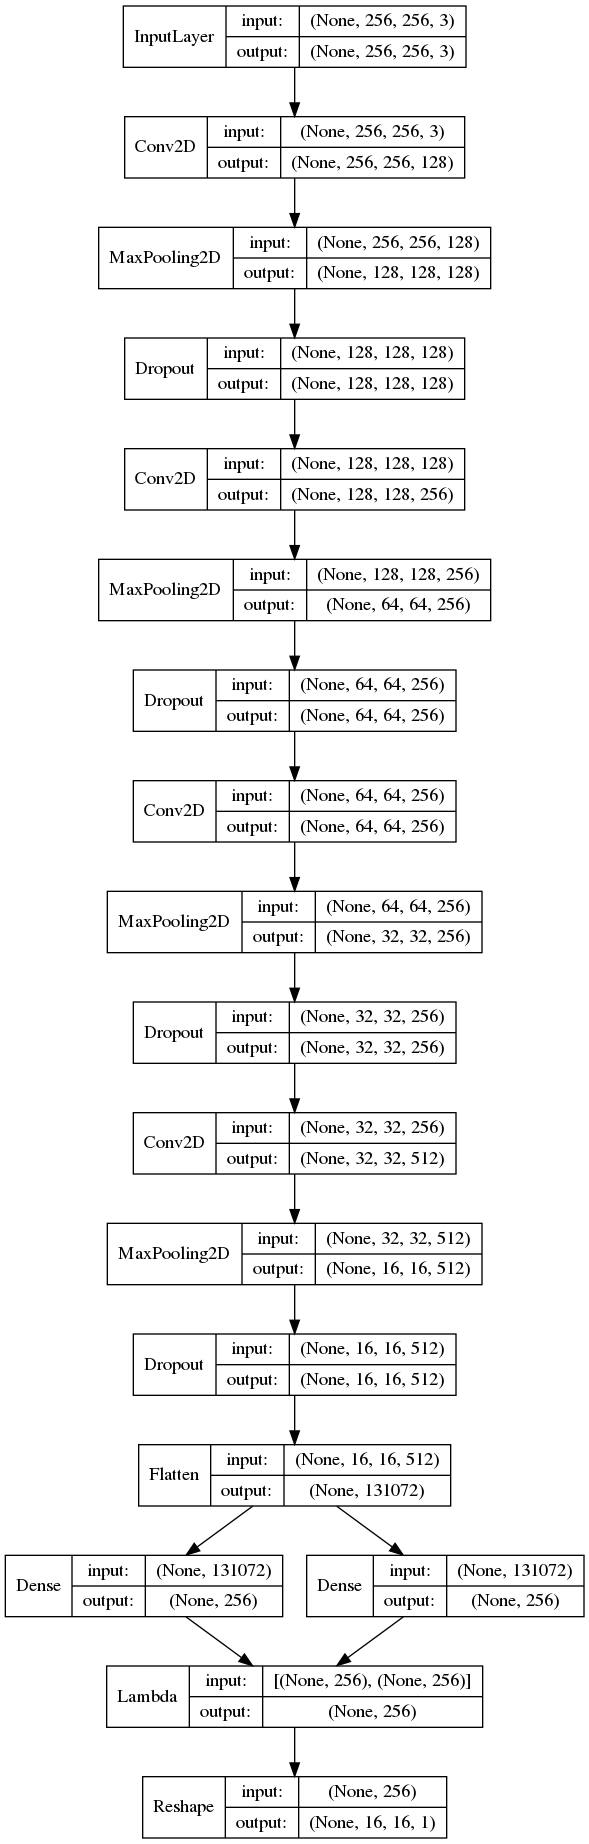
\includegraphics[scale=0.115]{encoder}
\end{flushleft}
\end{minipage}
\hfill
\begin{minipage}{0.1\textwidth}
\begin{center}
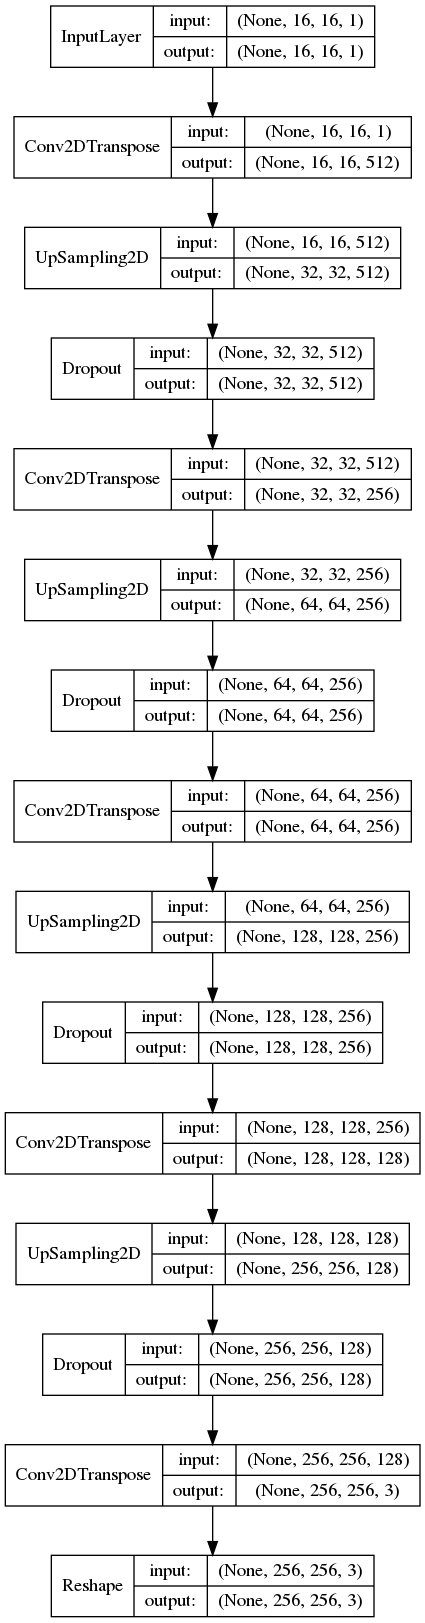
\includegraphics[scale=0.12]{decoder}
\end{center}
\end{minipage}
\hfill
\begin{minipage}{0.4\textwidth}
\begin{flushleft}
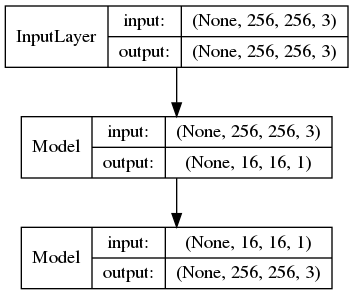
\includegraphics[scale=0.35]{autoencoder}
\end{flushleft}
\end{minipage}

\end{frame}

\subsection{Скорость обучения}

\begin{frame}{Применение вариационных автоэнкодеров к задаче}{Скорость обучения}

\begin{figure}[t]
\center{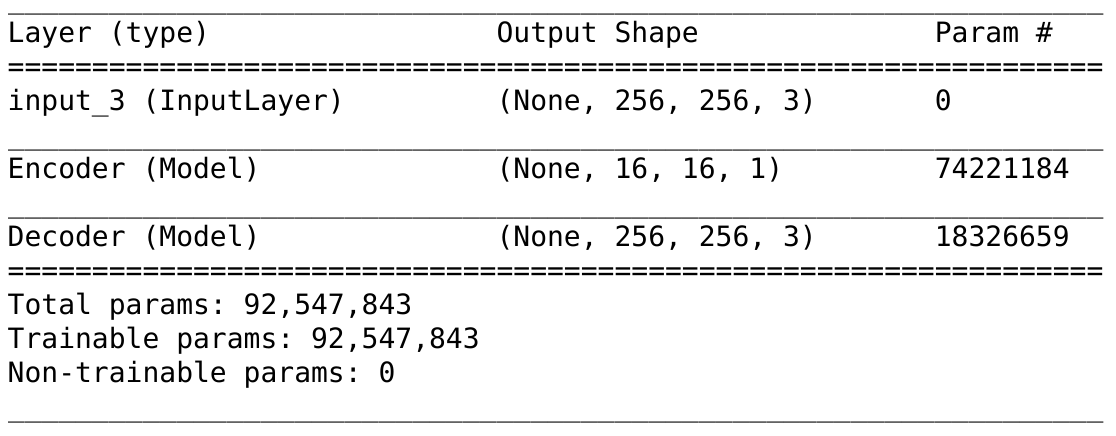
\includegraphics[scale=0.2]{vae_summary}}
\label{fig:vae}
\end{figure}

Используемые вычислительные и программные ресурсы:
\begin{itemize}
\item CPU: Intel i7-4770K, RAM: 16 Gb
\item GPU: Nvidia GTX 1080Ti 11 Gb
\item System: Linux Mint 18.2 Sonya x86\_64
\item Realisation: Keras(2.1.3) + Tensorflow(1.1.0) + CuDNN(7.1)
\end{itemize}

Время обучения одной эпохи на наборе из 154 644 изображений составляет 5 часов 7 минуты 23 секунды.
Оптимальное количество эпох - от 3 (15 часов).

\end{frame}

\subsection{Пример работы}

\begin{frame}{Применение вариационных автоэнкодеров к задаче}{Пример работы вариационного автоэнкодера}

\begin{minipage}{0.3\textwidth}
\begin{flushleft}
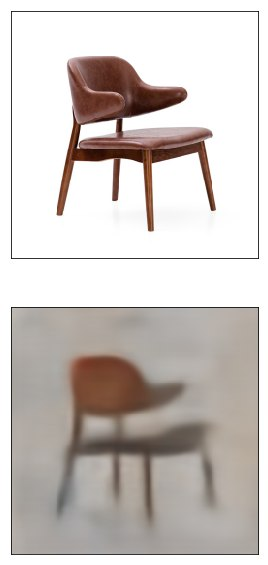
\includegraphics[scale=0.37]{stul}
\end{flushleft}
\end{minipage}
\hfill
\begin{minipage}{0.5\textwidth}
\begin{flushleft}
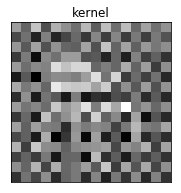
\includegraphics[scale=0.5]{stul_kernel}
\end{flushleft}
\end{minipage}

\end{frame}

\begin{frame}{Применение вариационных автоэнкодеров к задаче}{Пример работы вариационного автоэнкодера}

\begin{minipage}{0.3\textwidth}
\begin{flushleft}
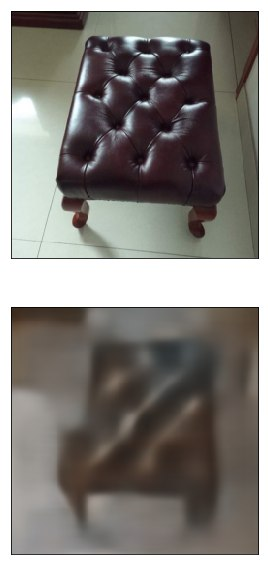
\includegraphics[scale=0.37]{sit}
\end{flushleft}
\end{minipage}
\hfill
\begin{minipage}{0.5\textwidth}
\begin{flushleft}
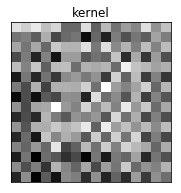
\includegraphics[scale=0.5]{sit_kernel}
\end{flushleft}
\end{minipage}

\end{frame}

\subsection{Кластеризация}

\begin{frame}{Применение вариационных автоэнкодеров к задаче}{Кластеризация}

Построим множество $H$ следующим образом:
\begin{equation}\label{eq:H}
H = \{g(x) | x \in X\},
\end{equation}
где $X$ - множество ~(\ref{eq:X}), ~$g$ - вариационный автоэнкодер. \par\medskip
Теперь понизим размерность множества H с помощью метода главных компонент (PCA) или алгоритма распределенного стохастического выделения соседей (t-SNE):
\begin{equation}\label{eq:hH}
\hat{H} = \text{t-SNE}(H), ~\forall h \in \hat{H} \Rightarrow dim(h) = 2
\end{equation}

К множеству $\hat{H}$ можно применять классические алгоритмы кластеризации данных, к примеру $k$-средних, предварительно выбрав количество классов.

\end{frame}

\begin{frame}{Применение вариационных автоэнкодеров к задаче}{Кластеризация}{Сравнение PCA и t-SNE}

\begin{figure}[h]{PCA}
\center{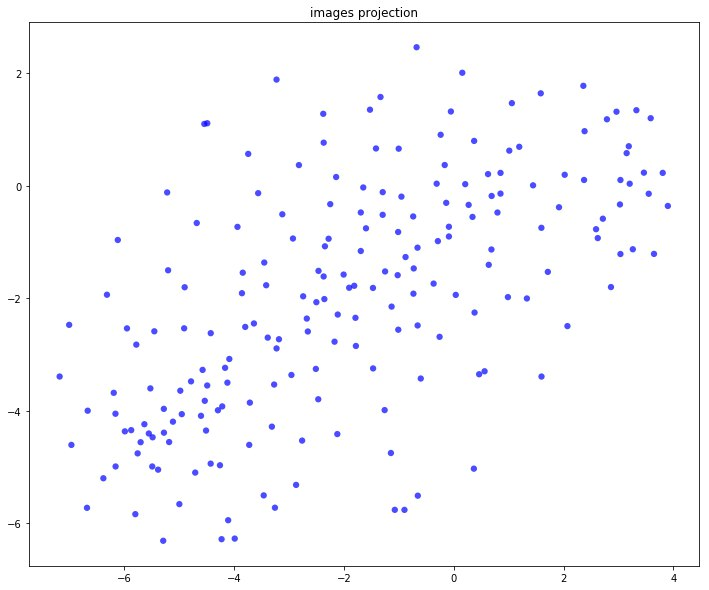
\includegraphics[scale=0.3]{pca}}
\label{fig:images_pca}
\end{figure}

\end{frame}

\begin{frame}{Применение вариационных автоэнкодеров к задаче}{Кластеризация}{Сравнение PCA и t-SNE}

\begin{figure}[h]{t-SNE}
\center{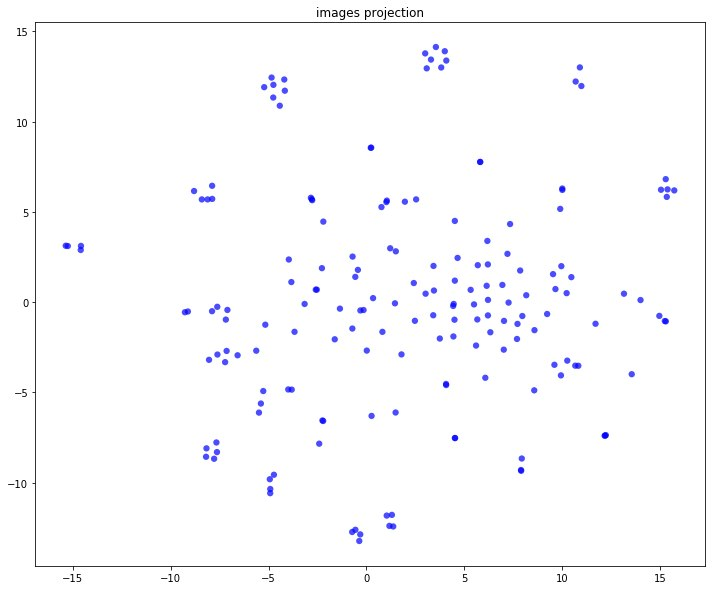
\includegraphics[scale=0.3]{images_p}}
\label{fig:images_t_sne}
\end{figure}

\end{frame}

\subsection{Поиск похожих по визуальному подобию}

\begin{frame}{Применение вариационных автоэнкодеров к задаче}{Поиск похожих по визуальному подобию}

Пусть $H$, как и в ~(\ref{eq:H}): $$H = \{g(x) | x \in X\}$$
Подействуем энкодером на входное изображение: $$h_{input} = g(I_{input})$$
Теперь найдем элементы множества $S$, это будут $M$-ближайших элемента из множества $H$ по евклидовой метрике.

\end{frame}

\section{Список литературы}

\begin{frame}{Список литературы}
\bibliographystyle{abbrv}
\bibliography{biblio}
\nocite{*}
\end{frame}

\end{document}